%
\documentclass[10pt,a4paper]{article}


\usepackage{array}
\usepackage{subfigure}
\usepackage{graphicx}
\usepackage{amssymb}
\usepackage{amsmath}
\usepackage{cite}
\usepackage{color}
\usepackage{url}
\usepackage[lined,linesnumbered,ruled,norelsize]{algorithm2e}
\usepackage{listings}
\lstset{
  language=Octave, 
  basicstyle=\footnotesize, 
  frame=single, 
  showspaces=false, 
  showstringspaces=false}
\date{}




\begin{document}

\title{Technical Report 1}

\maketitle

\section{Linear Regression}
%
  We implement linear regression according to the following model
  %
  \begin{equation}
    h_{\theta}(x) = \theta^Tx = \sum_{i=0}^n \theta_i x_i, \label{eqn:hypo}
  \end{equation}
  %
  and the batch gradient descent update rule is
  %
  \begin{equation}
    \theta_j := \theta_j - \alpha \frac{1}{m} \sum_{i=1}^m (h_\theta(x^{(i)}) - y^{(i)}) x^{(i)}_j \label{eqn:update}
  \end{equation}
  %
  where $j = 0, 1$ in our case.

  After the first iteration, we have 
  %
  \[ \theta_0 = 0.0745, ~~~~ \theta_1 = 0.3800\]
  %
  The gradient descent algorithm runs for about 1500 iteration, and the final values of $\theta_0$ and $\theta_1$ are 0.7502 and 0.0639, respectively. We plot the resulting straight line as well as the given data in Fig.~\ref{fig:lr}
  %
  \begin{figure}[htb!]
  \centering
    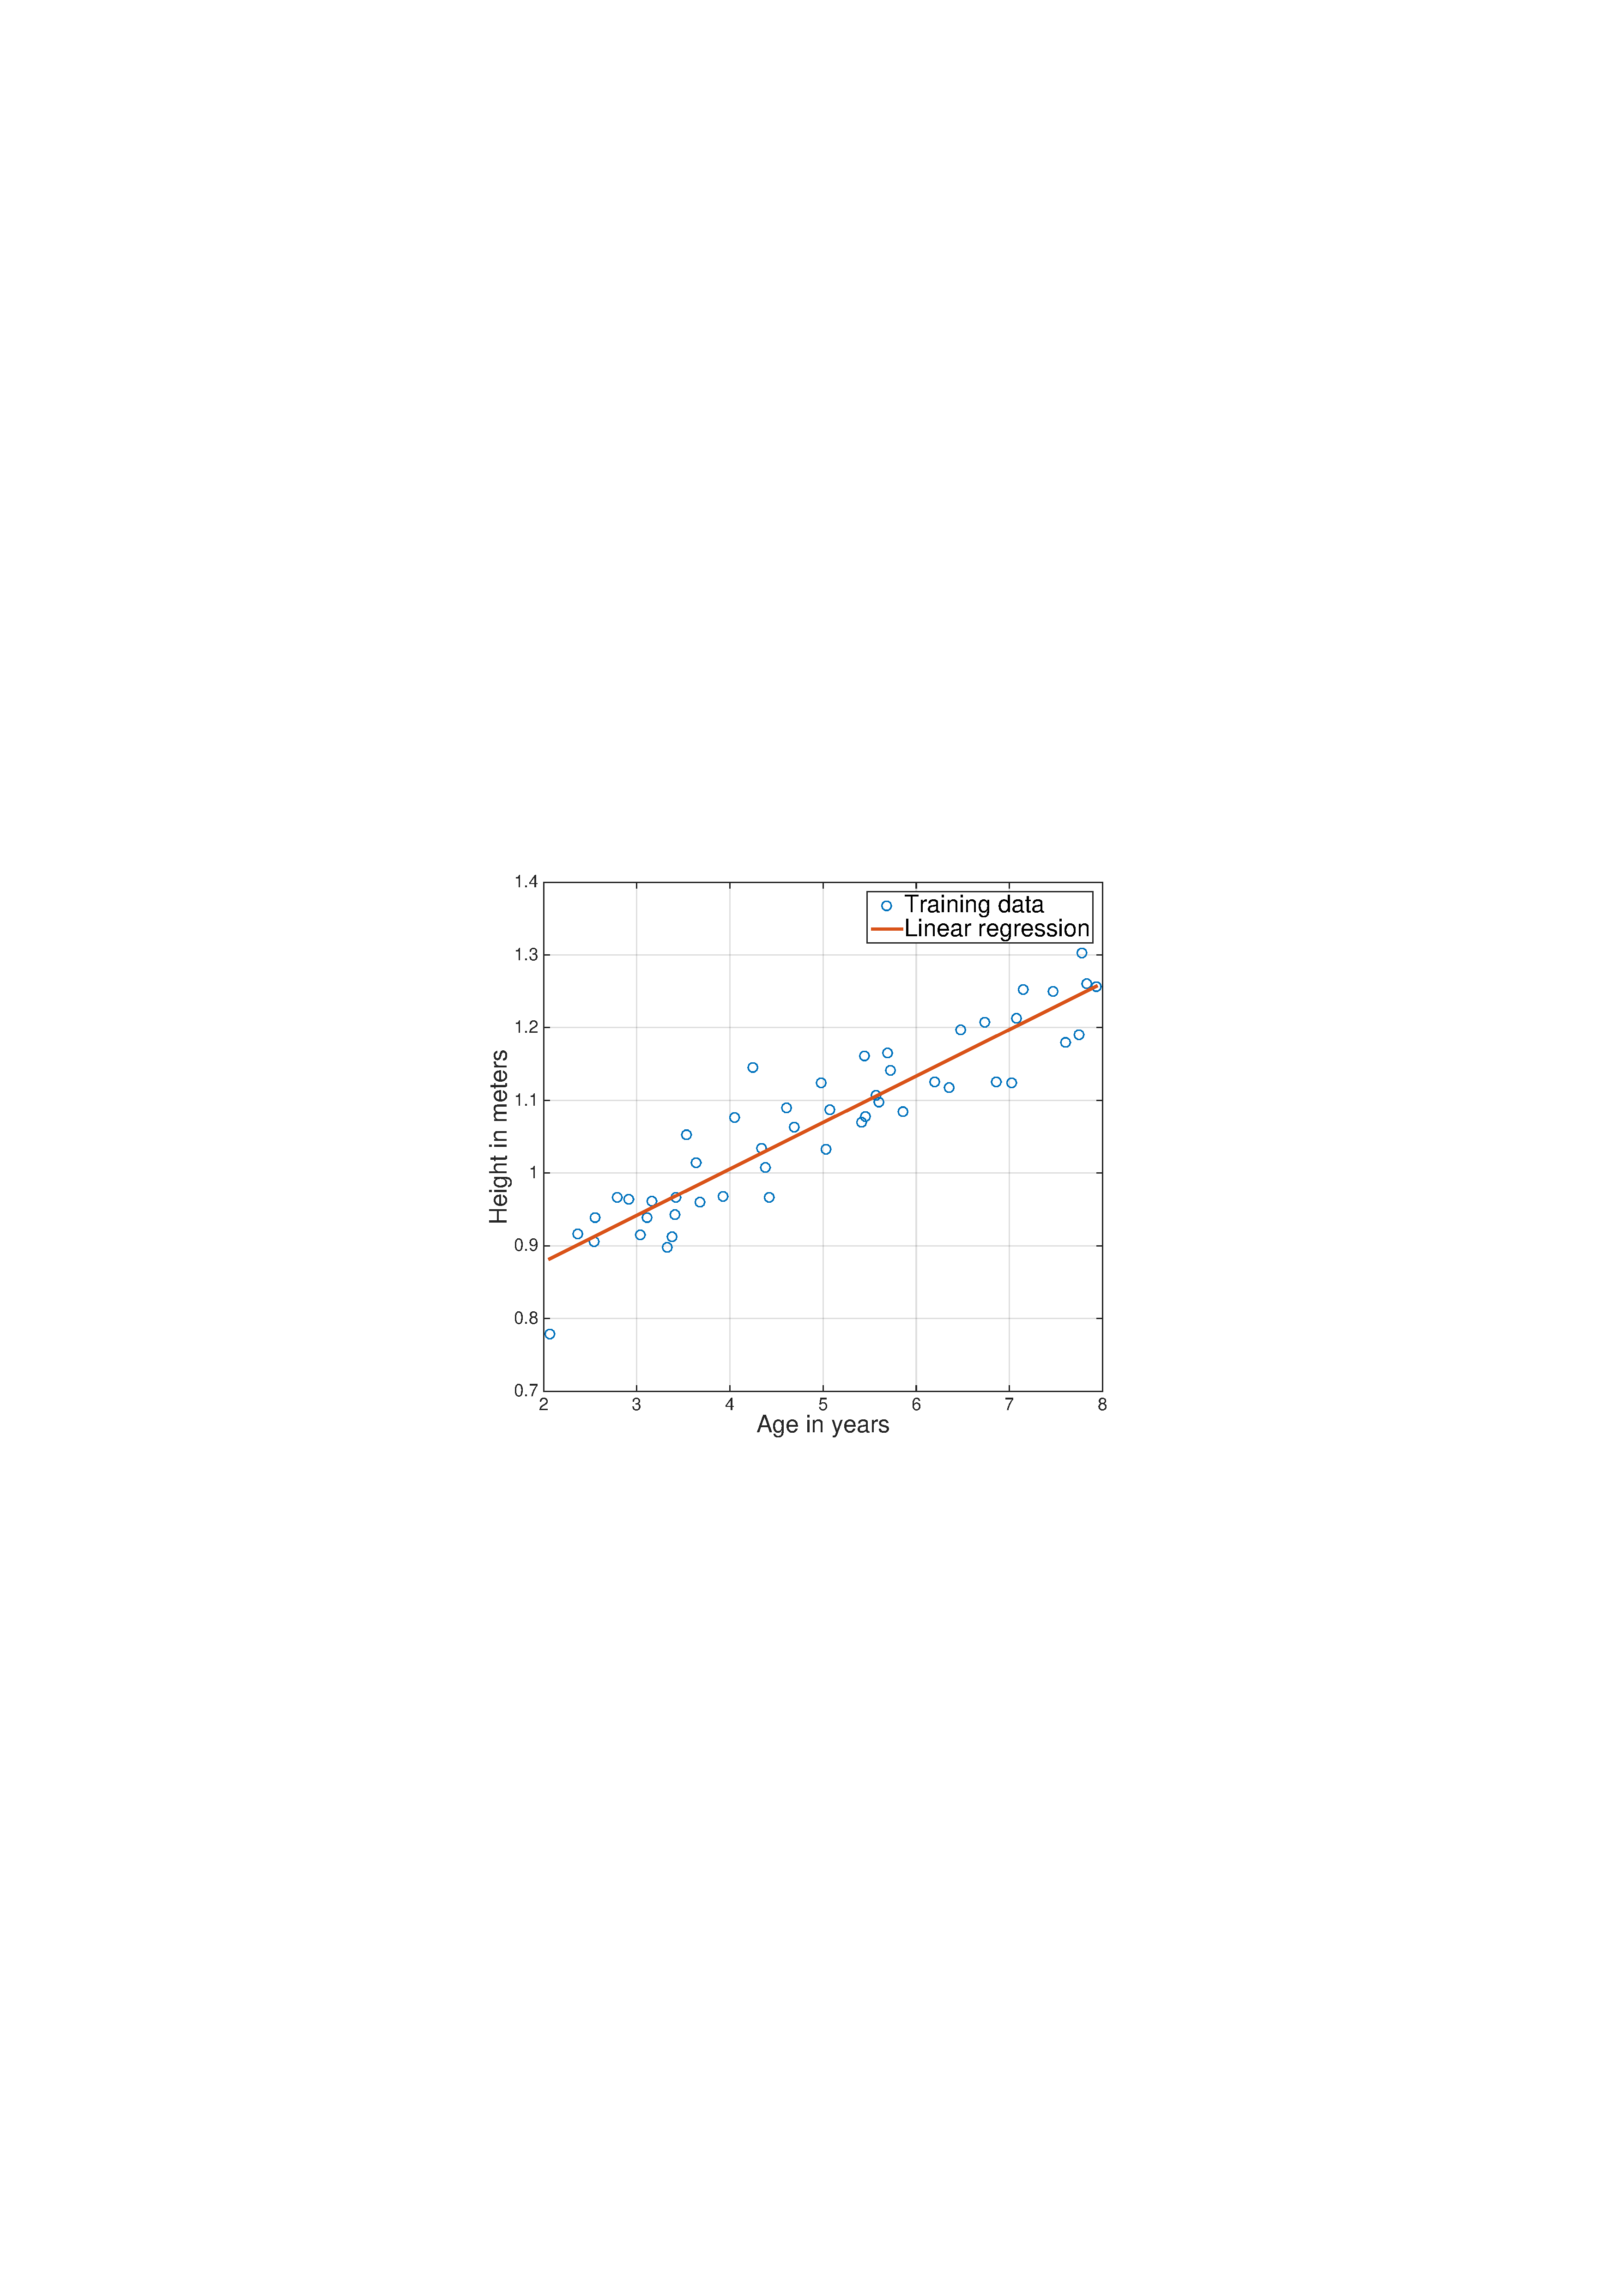
\includegraphics[width=.55\columnwidth]{lab1_lr} \\ %\vspace{1ex}
  \caption{The straight line fitting to the given data.}
  \label{fig:lr}
  \end{figure}

  Being aware of $\theta$, we can make predictions according to Equation~(\ref{eqn:hypo}). For example, given two boys of age 3.5 and age 7, their heights are 0.9737 meters and 1.1975 meters, respectively.



\section{Understanding $J$}
%
  The function $J(\theta)$ is visualized by a surface plot, as shown in Fig.~\ref{fig:surf}. It is demonstrated that, $J(\theta)$ has a global minimum with respect to $\theta$.
  %
  \begin{figure}[htb!]
  \centering
    \includegraphics[width=.7\columnwidth]{lab1_surf} \\ %\vspace{1ex}
  \caption{Visualizing $J(\theta)$.}
  \label{fig:surf}
  \end{figure}

  To illustrate the relationship between $J(\theta)$ and $\theta$, we also visualize $J(\theta)$ by a contour plot (see Fig.~\ref{fig:contour}. It is shown that, $J(\theta)$ approaches its minimum when $\theta_0=0.7502$ and $\theta_1=0.0639$
  %
  \begin{figure}[htb!]
  \centering
    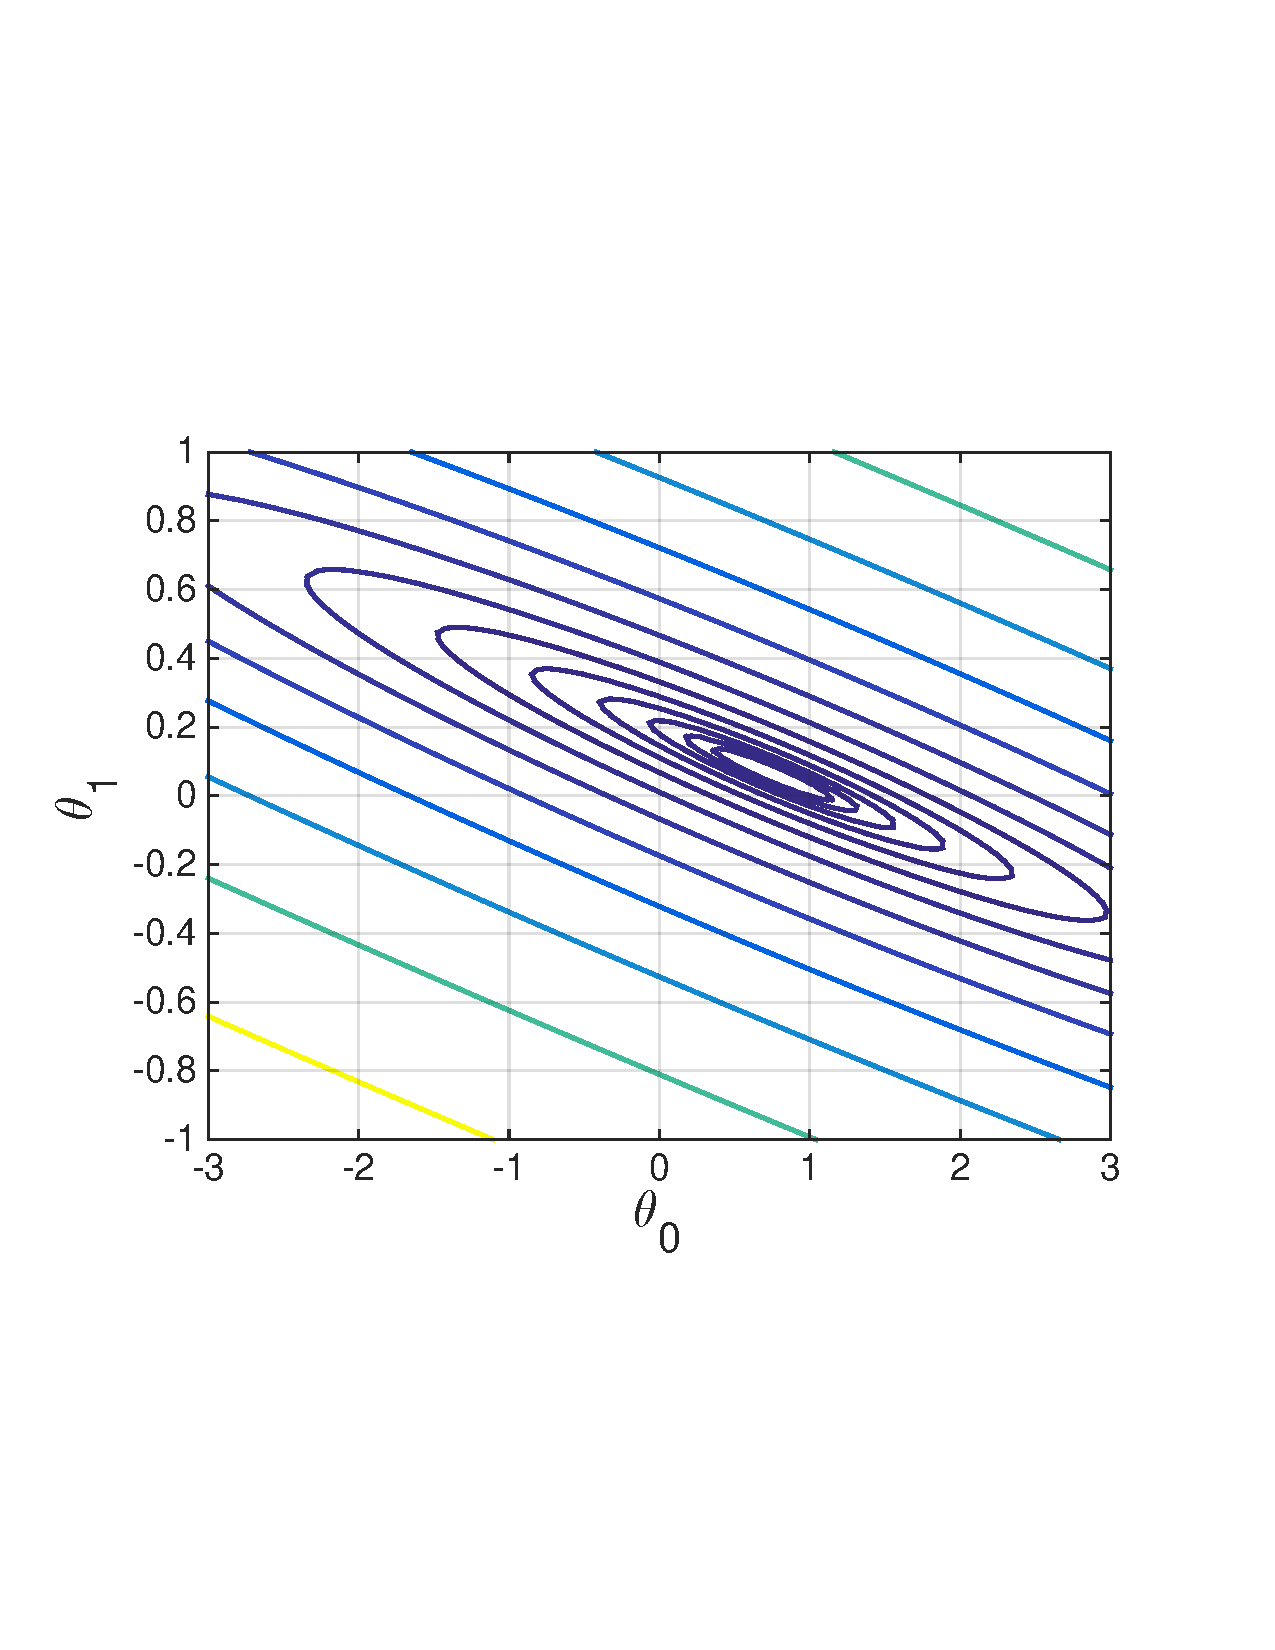
\includegraphics[width=.7\columnwidth]{lab1_contour} \\ %\vspace{1ex}
  \caption{Contour plot of $J(\theta)$.}
  \label{fig:contour}
  \end{figure}

\end{document}
\clearpage

\appendix
\section*{Appendix: Source Code}
%
  \begin{lstlisting}
% Initialization
clear all; close all; clc


% Load the data
x = load ('ex1x.dat') ;
y = load ('ex1y.dat') ;
m = length(y); % The number of training examples


% Plot the data
figure;
plot(x, y, 'o', 'MarkerSize', 10);
set(gca, 'FontSize', 18);
grid on;
ylabel('Height in meters', 'FontSize', 25);
xlabel('Age in years', 'FontSize',25);


%Gradient descent
x = [ones(m,1) x]; % Add a column of ones to x
theta = zeros(2, 1); % Initialize fitting parameters
MAX_ITR = 1500;
alpha = 0.07;

%
for it = 1:1:MAX_ITR
    grad = (1/m)*x'*(x*theta - y);
    theta = theta - alpha*grad;
    %theta = theta - alpha*(1/m)*x'*(x*theta - y)

end

% Print theta to screen
theta

% Plot the fitting line
hold on;
plot(x(:,2), x*theta, '-', 'LineWidth', 3);
legend({'Training data', 'Linear regression'}, 'FontSize', 25);
set(gcf, 'Position', [250 250 750 650]);

% Predict values for ages 3.5 and 7
predict1 = [1, 3.5]*theta
predict1 = [1, 7]*theta

% Calculate J matrix

% Grid over which we will calculate J
theta0_vals = linspace(-3, 3, 100);
theta1_vals = linspace(-1, 1, 100);

% Initialize J_vals
J_vals = zeros(length(theta0_vals), length(theta1_vals));

for i = 1:length(theta0_vals)
    for j = 1:length(theta1_vals)
	  t = [theta0_vals(i); theta1_vals(j)];    
	  J_vals(i,j) = (0.5/m) .* (x * t - y)' * (x * t - y);
    end
end

%

% Due to the rule of surf, we have to transpose J_vals
J_vals = J_vals';

% Surface plot
figure;
surf(theta0_vals, theta1_vals, J_vals)
set(gca, 'FontSize', 18);
xlabel('\theta_0', 'FontSize', 25); 
ylabel('\theta_1', 'FontSize', 25);
zlabel('J(\theta)', 'FontSize', 25);
colorbar;

% Contour plot
figure;
% Plot J_vals as 15 contours spaced logarithmically 
% between 0.01 and 100
contour(theta0_vals, theta1_vals, J_vals, logspace(-2, 2, 15));
set(gca, 'FontSize', 18);
xlabel('\theta_0', 'FontSize', 25);
ylabel('\theta_1', 'FontSize', 25);
grid on;


  \end{lstlisting}
  %


